% Author: Vitaly Parnas
\documentclass{article}

\usepackage{tikz}
\usepackage[paperheight=16in,paperwidth=16in,margin=1in,heightrounded]{geometry}
\usepackage{amsmath}
\usetikzlibrary{mindmap,trees}
\usepackage{verbatim}
\graphicspath{ {images/} }

\begin{document}
\pagestyle{empty}

\begin{comment}
:Title: Computability Mind Map
:Tags: Manual, Mindmap

| Author: Vitaly Parnas
| Source: Computability Georgia Tech CS6605 Course Material
\end{comment}

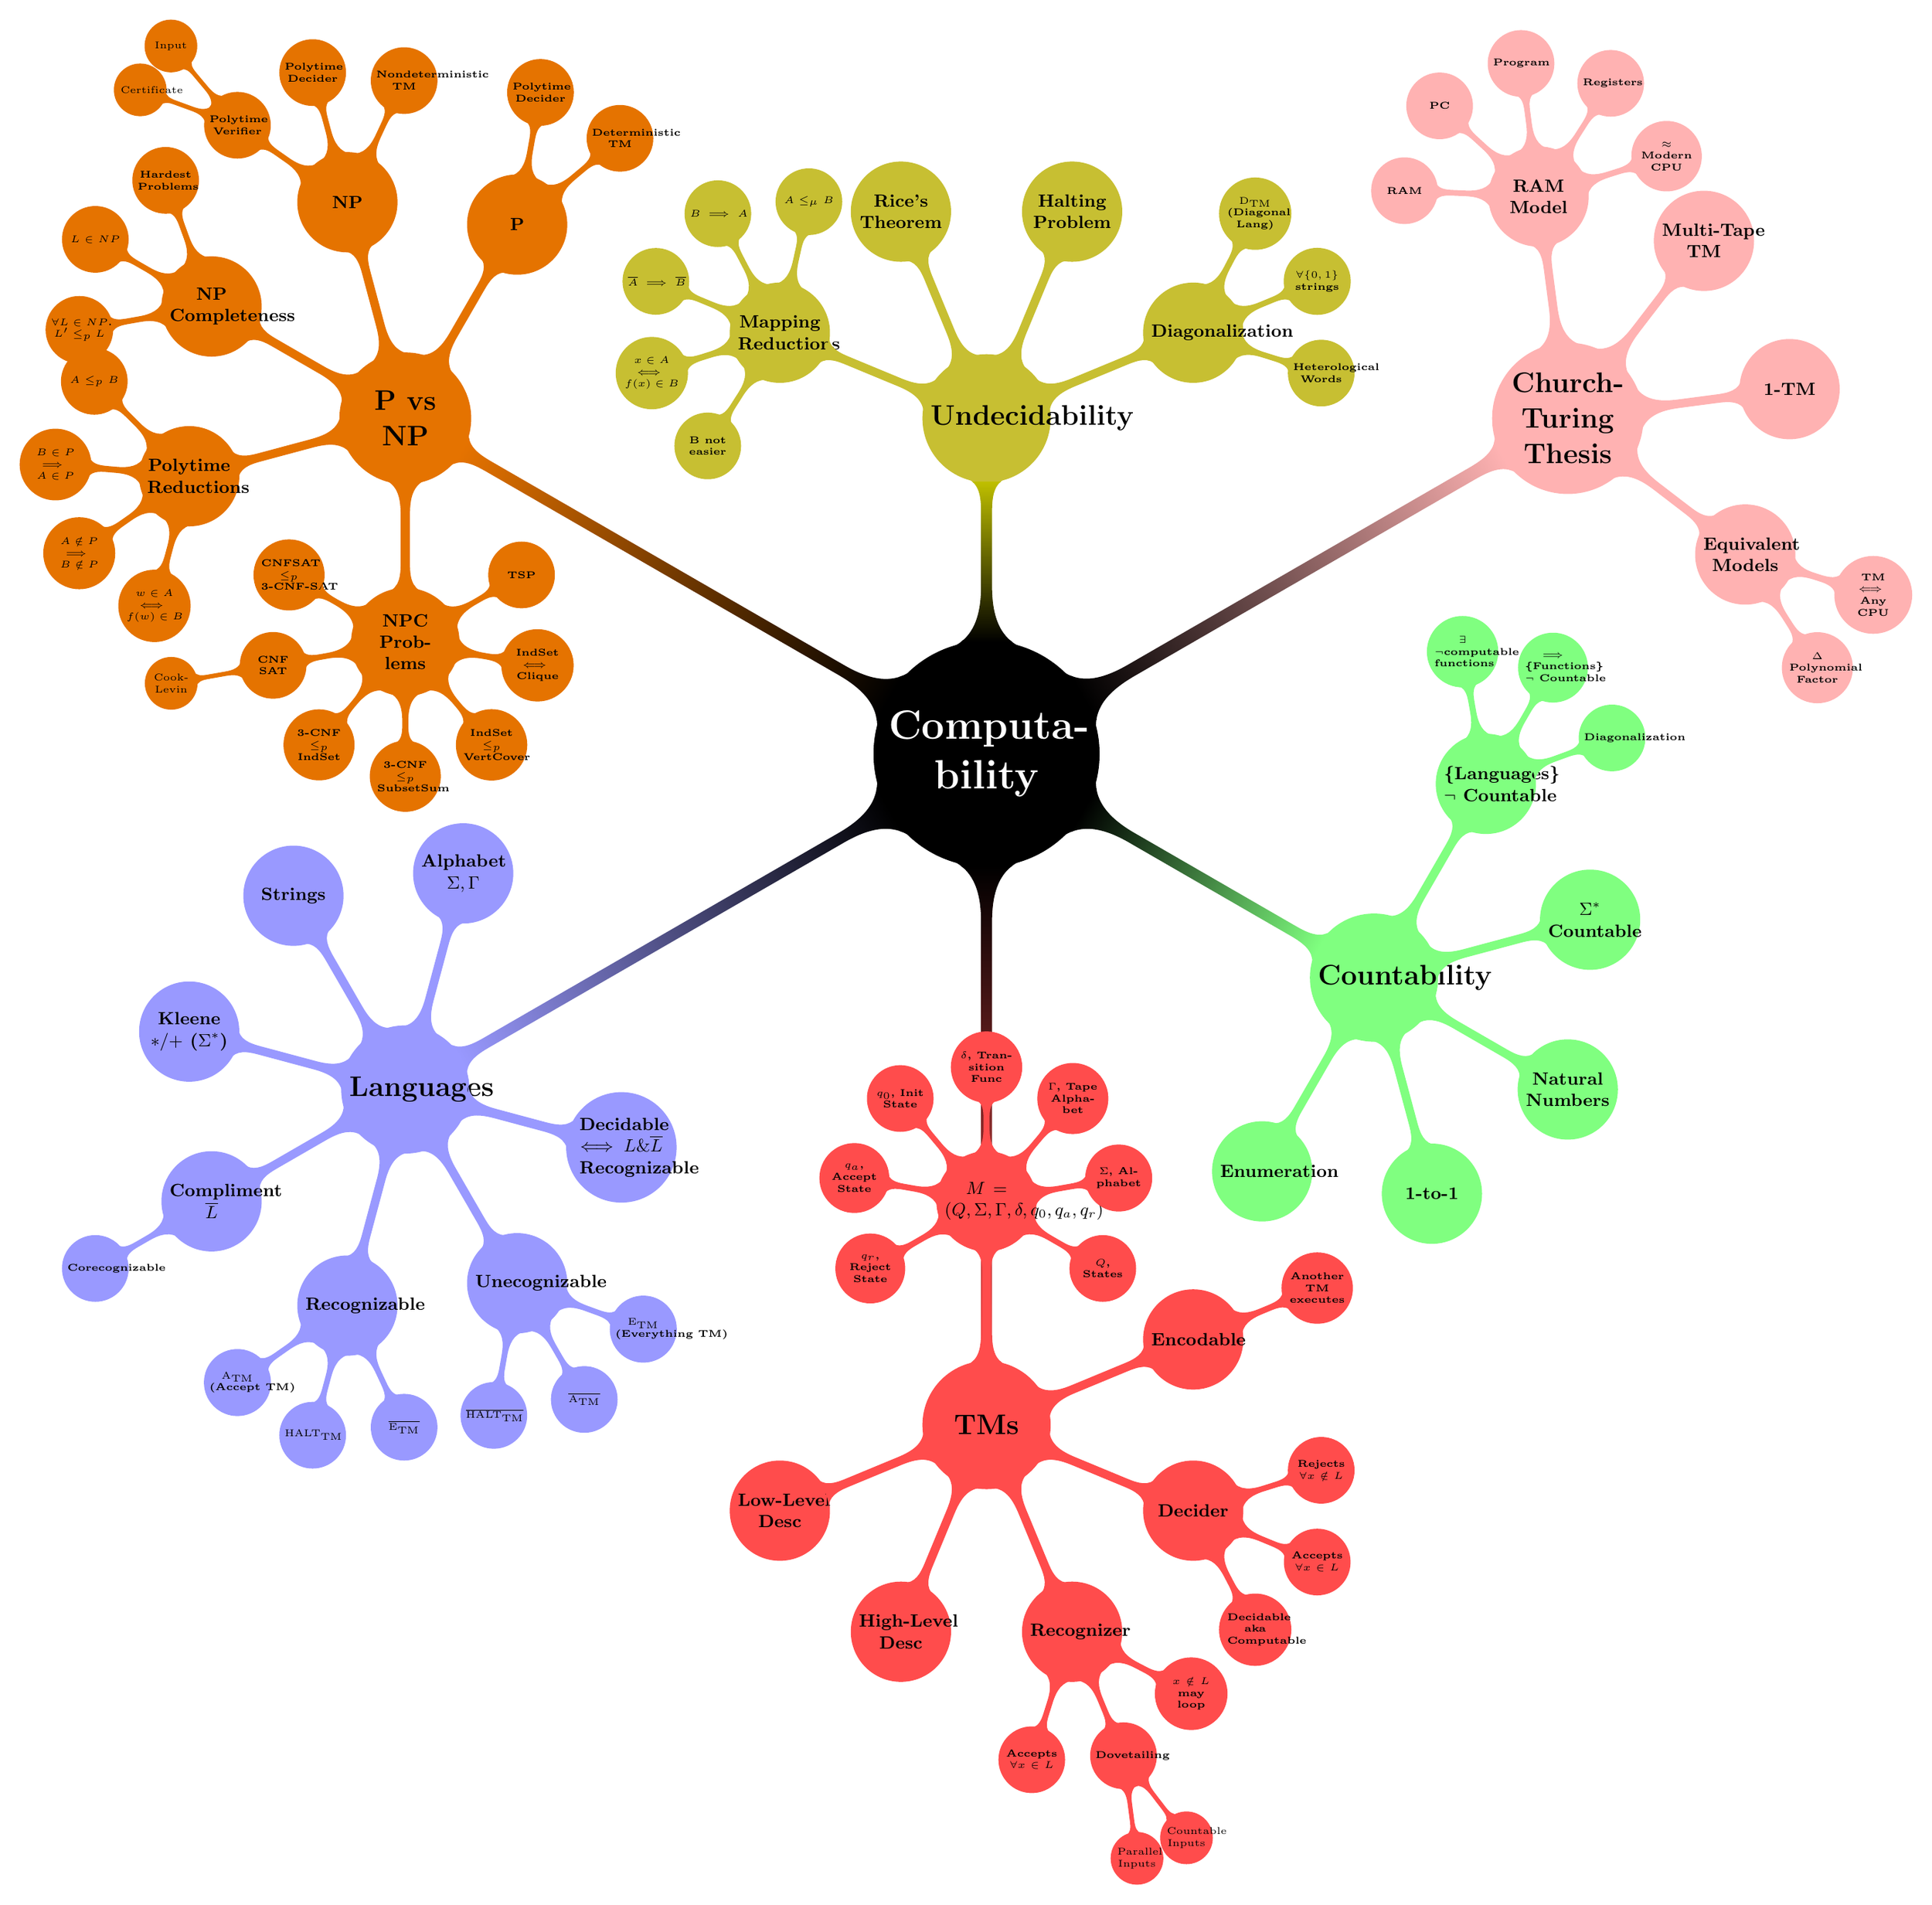
\begin{tikzpicture}[mindmap, grow cyclic, every node/.style=concept,
    concept color=black,text=white,
    level 1/.append style={font=\Large\bfseries,level distance=12cm,sibling angle=60},
    level 2/.append style={font=\small\bfseries,level distance=4cm,sibling angle=45},
    level 3/.append style ={font=\tiny\bfseries,sibling angle=40},
    nucleus/.style= {concept, font=\huge\bfseries},
    ]

    % mbox content remains on one line
    \node [nucleus] {Computa-bility}
    child[concept color=blue!40!white,text=black] { node {Languages}
        child{ node {Alphabet $\Sigma, \Gamma$} }
        child{ node {Strings}}
        child{ node {Kleene $*/+$ ($\Sigma^{*}$)}}
        child{ node {Compliment $\overline{L}$}
            child{ node {Corecognizable}}
        }
        child{ node {Recognizable}
            child{ node {$\mathrm{A_{TM}}$ (\mbox{Accept TM})}}
            child{ node {$\mathrm{HALT_{TM}}$}}
            child{ node {$\mathrm{\overline{E_{TM}}}$}}
        }
        child{ node {Unecognizable}
            child{ node {$\overline{\mathrm{HALT_{TM}}}$}}
            child{ node {$\overline{\mathrm{A_{TM}}}$}}
            child{ node {$\mathrm{E_{TM}}$ (\mbox{Everything TM})}}
        }
        child{ node {Decidable $\iff L \& \overline{L}$ \mbox{Recognizable}} }
    }
    child[concept color=red!70!white,text=black] { node {TMs}
        child[sibling angle=72]{ node {$M=(Q,\Sigma,\Gamma,\delta,q_0,q_a,q_r)$} 
            child { node {$Q$, States} }
            child { node {$\Sigma$, Alphabet} }
            child { node {$\Gamma$, Tape Alphabet} }
            child { node {$\delta$, Transition Func} }
            child { node {$q_0$, Init State} }
            child { node {$q_a$, Accept State} }
            child { node {$q_r$, Reject State} }
        }
        child { node {\mbox{Low-Level} Desc} }
        child { node {\mbox{High-Level} Desc} }
        child { node {Recognizer} 
            child { node {Accepts $\forall x \in L$} }
            child { node {Dovetailing} 
                child { node {Parallel Inputs}}
                child { node {Countable Inputs}}
            }
            child { node {$x \notin L$ may loop} }
        }
        child { node {Decider} 
            child { node {Decidable aka \mbox{Computable}} }
            child { node {Accepts $\forall x \in L$} }
            child { node {Rejects $\forall x \notin L$} }
        }
        child { node {Encodable} 
            child { node {Another TM executes} }
        }
    }
    child[concept color=green!50!white,text=black,level distance=8cm] { node {Countability}
        child{ node {Enumeration} }
        child{ node {1-to-1} }
        child{ node {Natural Numbers} }
        child{ node {$\Sigma^{*}$ \mbox{Countable}} }
        child{ node {\{Languages\} \mbox{$\neg$ Countable}} 
            child { node {Diagonalization} }
            child { node {$\implies$ \{Functions\} \mbox{$\neg$ Countable}} }
            child { node {$\exists$ \mbox{$\neg$computable} \mbox{functions}} }
        }
    }
    child[concept color=red!30!white,text=black] { node {Church-Turing Thesis}
        child{ node {Equivalent Models} 
            child{ node {$\Delta$ \mbox{Polynomial} Factor} }
            child{ node {TM $\iff$ Any CPU} }
        }
        child{ node {1-TM} }
        child{ node {\mbox{Multi-Tape} TM} }
        child{ node {RAM Model} 
            child{ node {$\approx$ Modern CPU} }
            child{ node {Registers} }
            child{ node {Program} }
            child{ node {PC} }
            child{ node {RAM} }
        }
    }
    child[concept color=yellow!75!black,text=black,level distance=6cm] { node {Undecidability}
        child{ node {Diagonalization} 
            child{ node {Heterological Words} }
            child{ node {$\forall \{0,1\}$ strings} }
            child{ node {$\mathrm{D_{TM}}$ (\mbox{Diagonal} Lang)}}
        }
        child{ node {Halting Problem} }
        child{ node {Rice's Theorem} }
        child{ node {Mapping \mbox{Reductions}} 
            child{ node {$A\leq_{\mu}B$} }
            child{ node {\mbox{$B \implies A$}} }
            child{ node {\mbox{$\overline{A} \implies \overline{B}$}} }
            child{ node {\mbox{$x \in A$} $\iff$ \mbox{$f(x) \in B$}} }
            child{ node {B not easier} }
        }
    }
    child[concept color=orange!90!black,text=black] { node {P vs NP}
        child{ node {P} 
            child{ node {Deterministic TM} }
            child{ node {Polytime Decider} }
        }
        child{ node {NP} 
            child{ node {Nondeterministic TM} }
            child{ node {Polytime Decider} }
            child{ node {Polytime Verifier} 
                child{ node {Input} }
                child{ node {Certificate} }
            }
        }
        child{ node {NP \mbox{Completeness}} 
            child{ node {Hardest \mbox{Problems}} }
            child{ node {$L \in NP$} }
            child{ node {\mbox{$\forall L \in NP$.} \mbox{$L' \leq_p L$}} }
        }
        child{ node {Polytime \mbox{Reductions}} 
            child{ node {$A\leq_{p}B$} }
            child{ node {\mbox{$B \in P$} $\implies$ \mbox{$A \in P$}} }
            child{ node {\mbox{$A \notin P$} $\implies$ \mbox{$B \notin P$}} }
            child{ node {\mbox{$w \in A$} $\iff$ \mbox{$f(w) \in B$}} }
        }
        child[sibling angle=60]{ node {NPC Problems} 
            child{ node {CNFSAT $\leq_p$ \mbox{3-CNF-SAT}} }
            child{ node {CNF SAT} 
                child{ node {Cook-Levin} }
            }
            child{ node {3-CNF $\leq_p$ IndSet} }
            child{ node {3-CNF $\leq_p$ \mbox{SubsetSum}} }
            child{ node {IndSet $\leq_p$ \mbox{VertCover}} }
            child{ node {IndSet $\iff$ Clique} }
            child{ node {TSP} }
        }
    }
    ;
\end{tikzpicture}
\end{document}
